The main high level components of the system are:

\begin{description}
\item[Database:] The system data layer; it includes all structures and entities responsible for data storage and management. No application logic is found at this level, apart from the DBMS one that must guarantee the correct functioning of the data structures while assuring the ACID properties of transactional databases.
\item[Application Server:] This layer encloses all the logic for the system applications, including the logic needed to interface with external systems and the key algorithms.
\item[Web Server:] This layer is in charge of providing web pages for the web-based application, and does not include any logic besides the basic request-response interaction one.
\item[Mobile Application:] The presentation layer dedicated to mobile devices; it communicates directly with the application server and only includes presentation logic.
\item[Web Browser:] The presentation layer dedicated to web browsers; it relies on the connection with the Web Server to obtain the pages to be rendered on the client.
\item[On-Board Application:] The presentation layer dedicated to the on-board computers applications; it communicates with the Application Server for the most part of the logic; however it also includes the logic needed to interface with the physical car systems and to perform ride-related actions/computations.
\end{description}

The described components are structured in four layers, as shown in Figure \ref{sys_layers}. Said figure also includes the interaction with external systems, that is intended to happen at the level of the Application Server.

The choice of separating the Application and Web Server layers allows greater scalability, since it allows the deployment on distinct physical tiers that can individually be optimized to perform their respective task.

\begin{figure}[H]
\begin{center}
		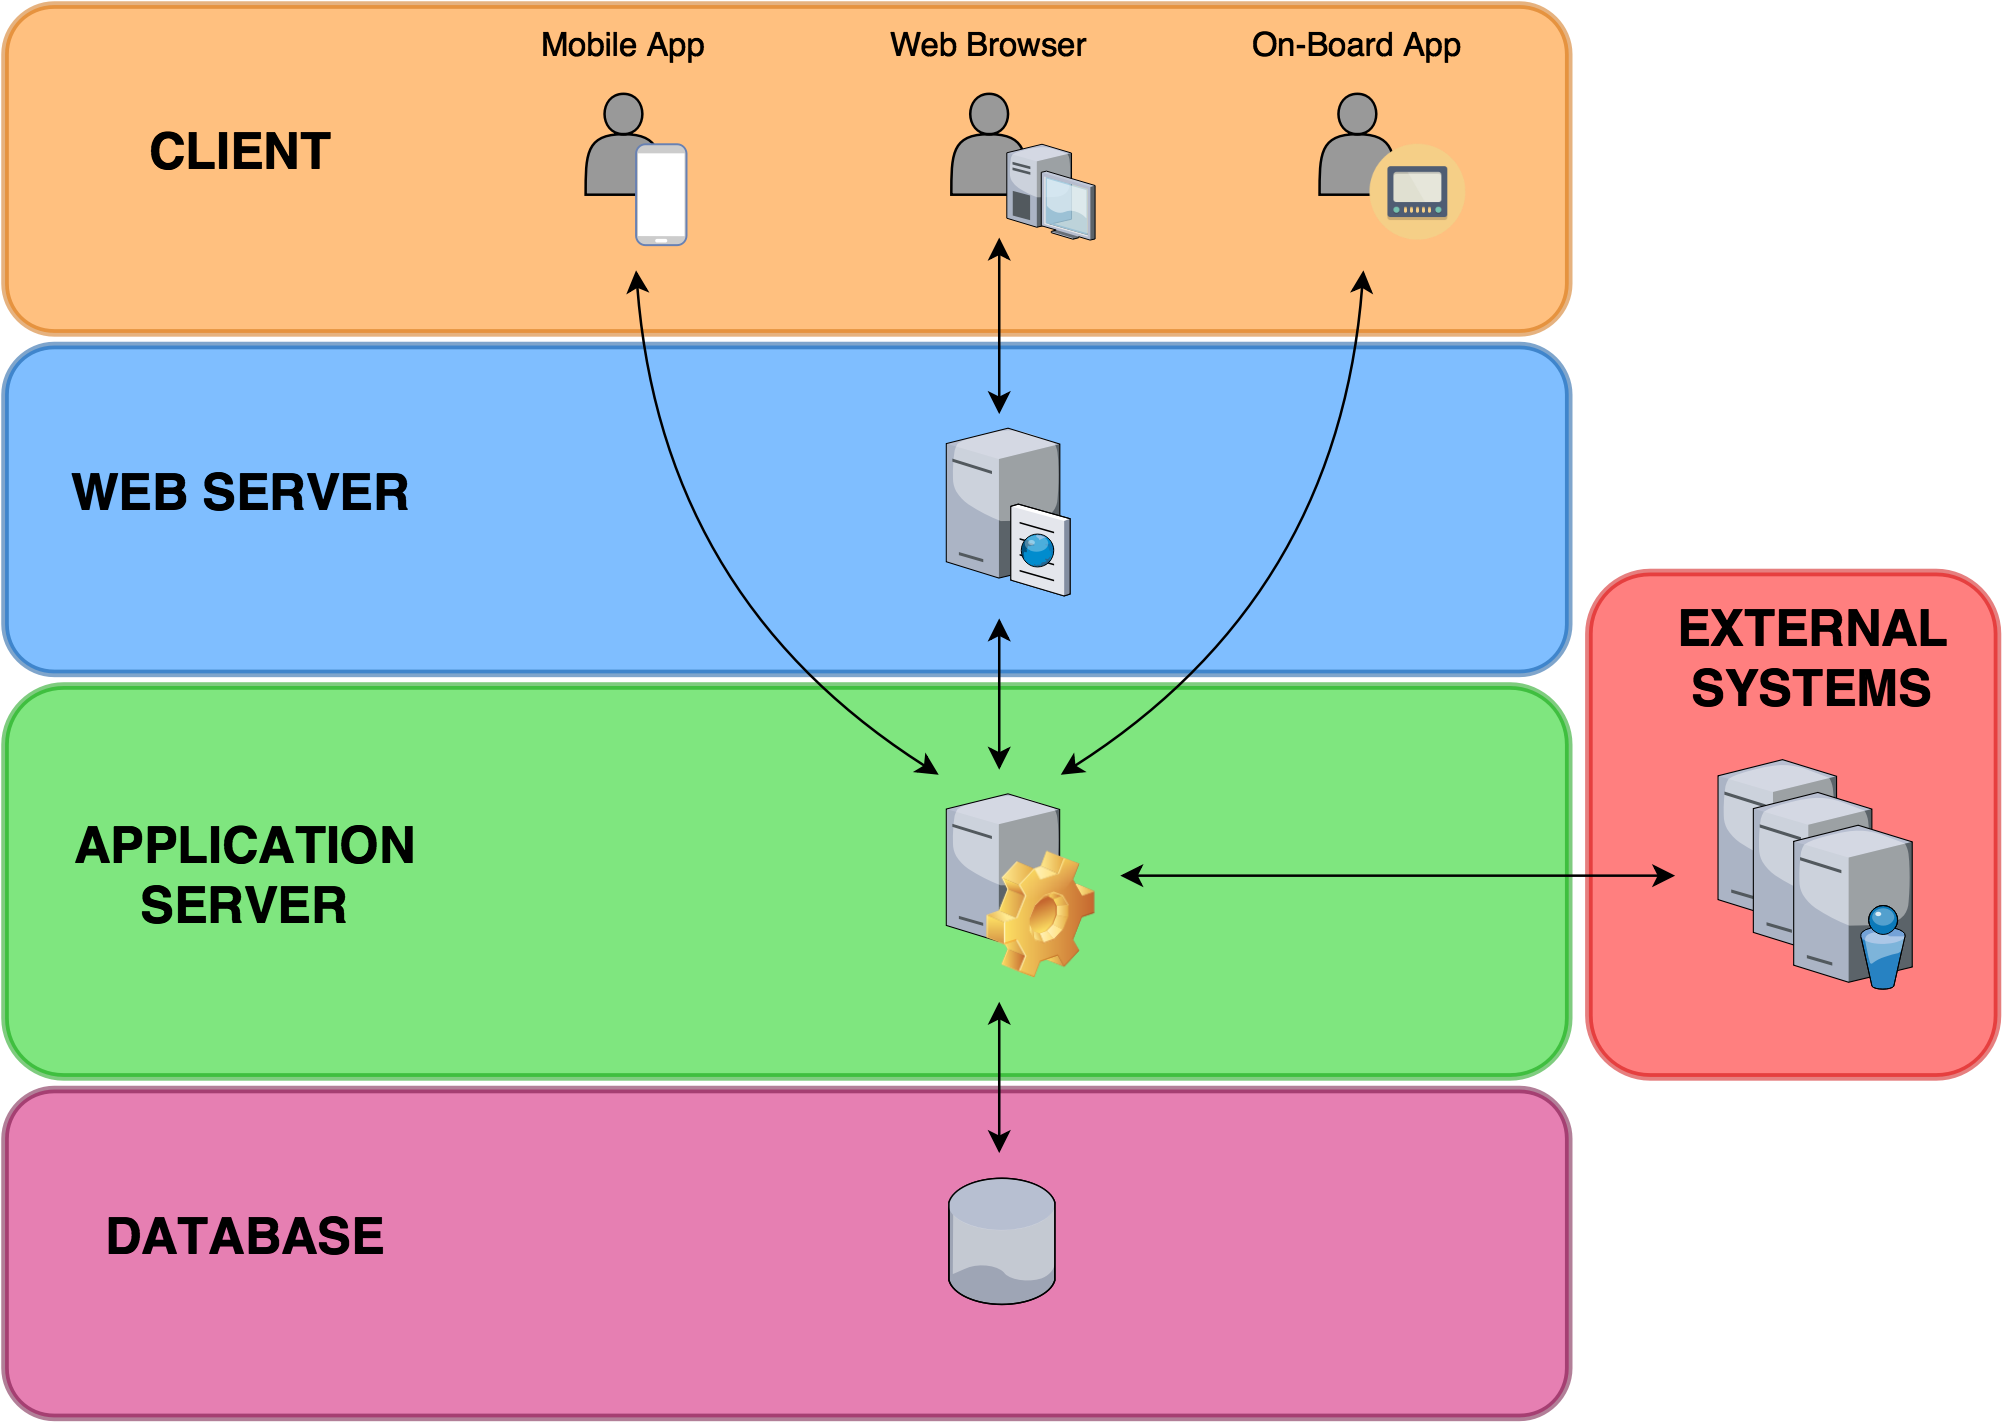
\includegraphics[width=\textwidth]{./arch_design/diagrams/system_layers.png}
		\caption{Layered structure of the system.}
		\label{sys_layers}
\end{center}
\end{figure}

The interaction among the main system components is shown in Figure \ref{sys_comps}. The diagram noticeably points out the interaction with the payment handler and the maintenance systems, meant to support the \emph{PowerEnJoy} service as stated in the RASD document~\cite{rasd}. Note that the web server and the application server are multi-threaded.

\begin{figure}[H]
\begin{center}
		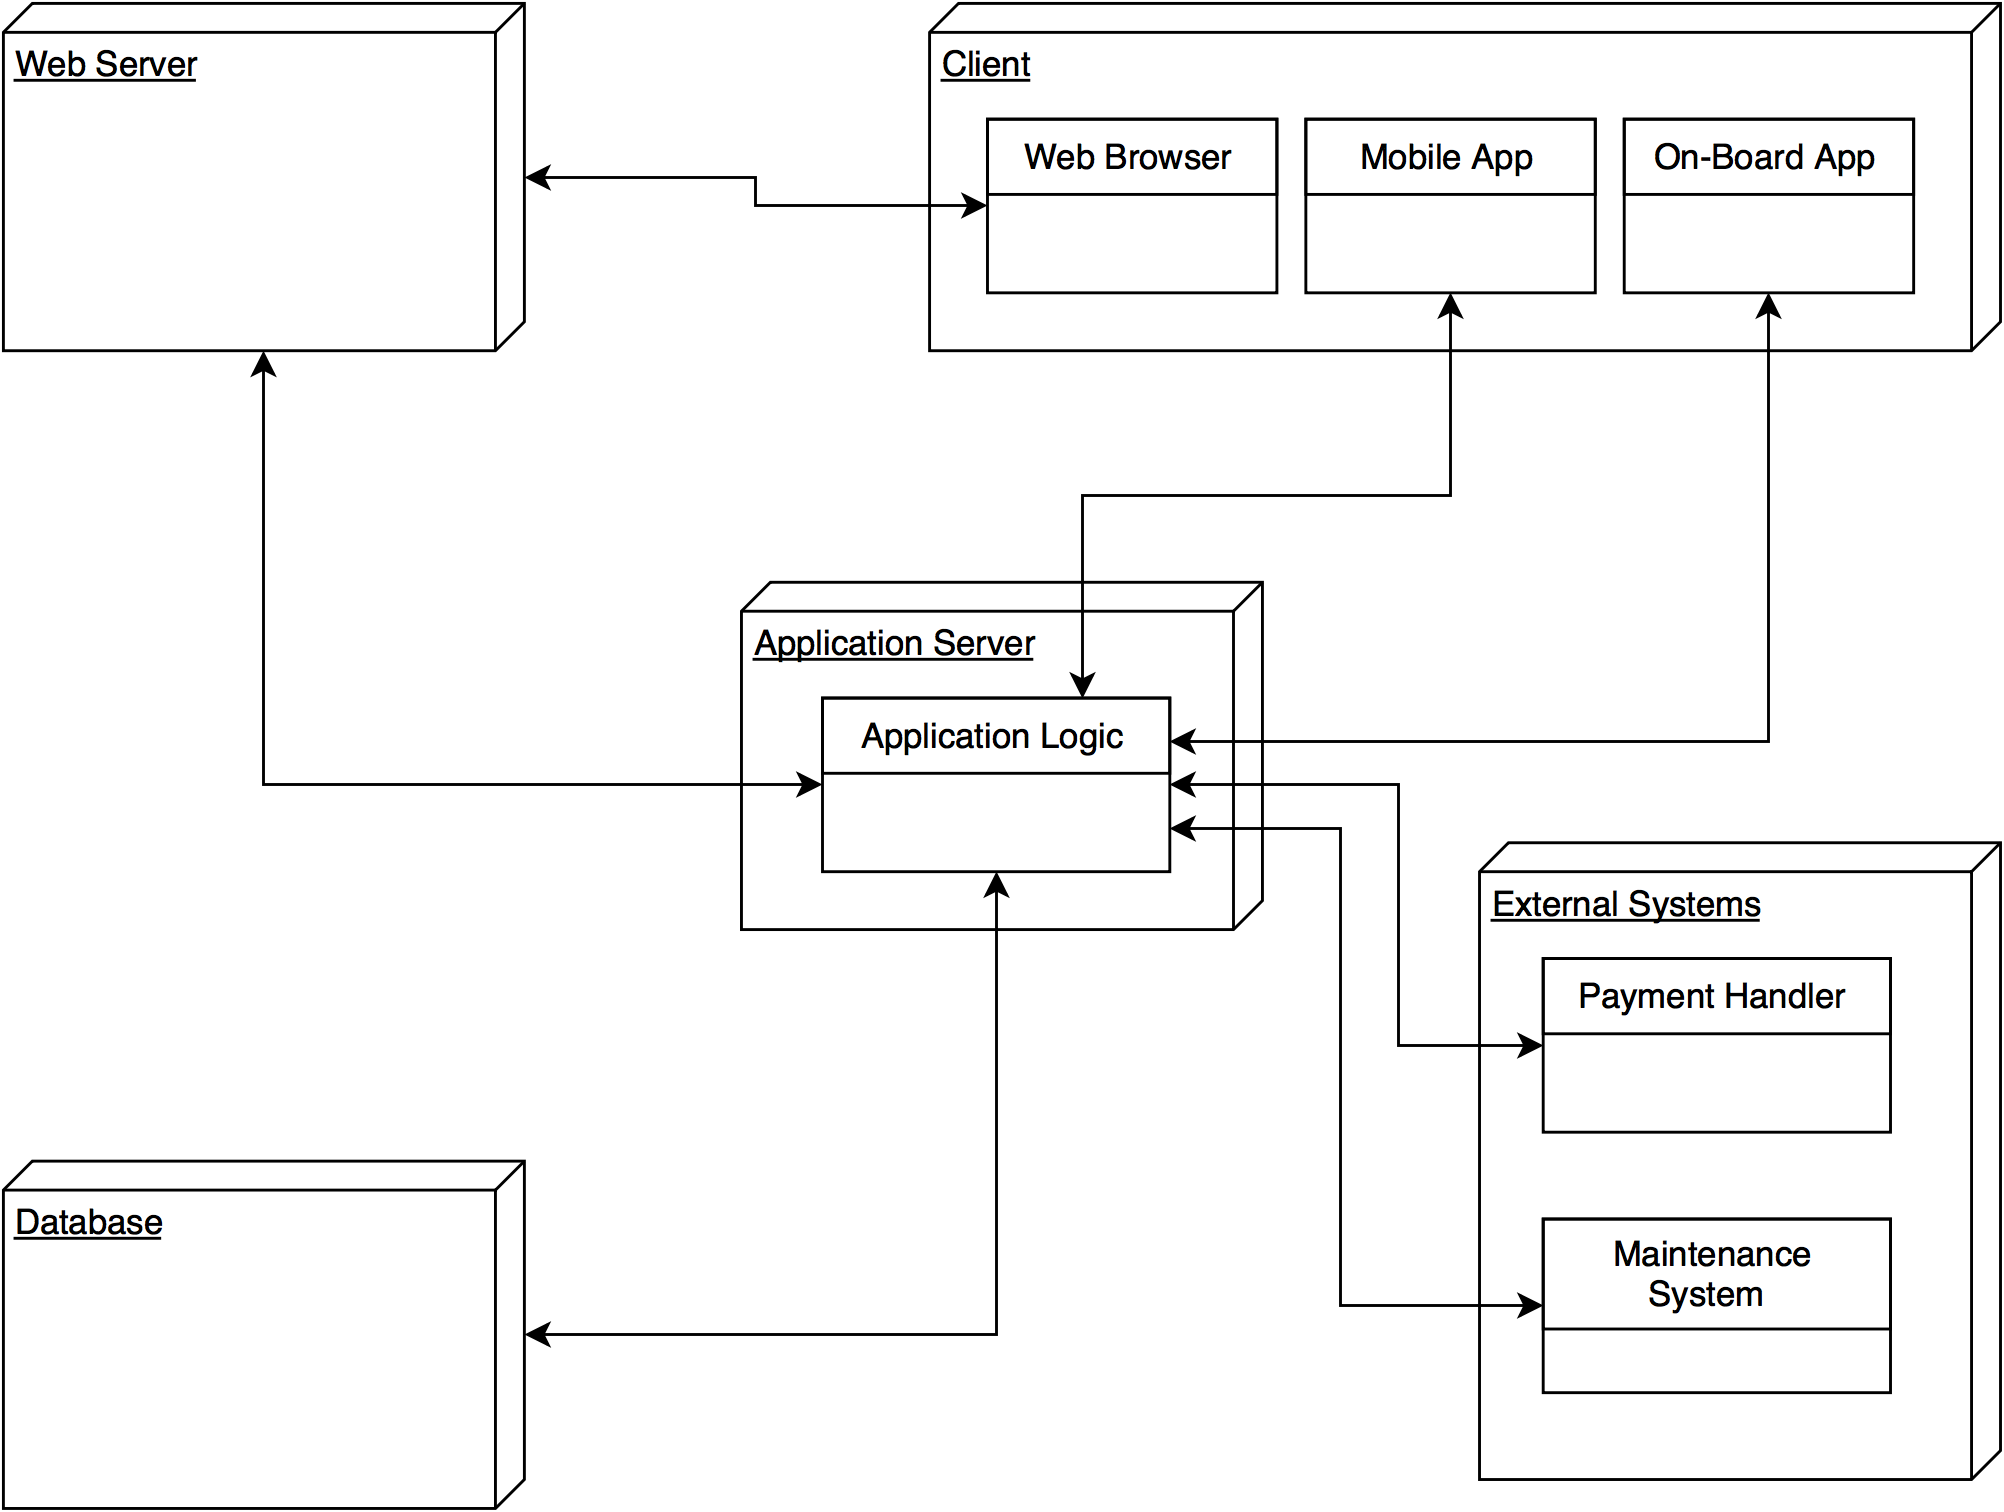
\includegraphics[width=0.9\textwidth]{./arch_design/diagrams/system_components.png}
		\caption{The high level components of the system.}
		\label{sys_comps}
\end{center}
\end{figure}